\section{Résultats}

\subsection{Extraction du SOS et du EOS}

\`A partir des profils temporels de NDVI obtenus par les 2 méthodes de lissage (HANTS et Whittaker), nous avons extrait le SOS et le EOS respectivement avec les seuils de 10, 20, 30 puis 50\% avant le MAX et 50, 60, 70 puis 80\% après le MAX. Nous avons calculé ensuite pour chacune des parcelles terrain, les écarts en nombre de jours entre les dates de semis et les SOS extraits puis entre les dates de récolte et les EOS estimés. En considérant ces écarts par sytème de culture, nous avons calculé 2 indicateurs statistiques : la racine carrée de l'erreur quadratique moyenne ou \acrshort{rmse} qui est un indicateur d'écart entre valeurs observées et valeurs prédites et le coefficient de variation ou \acrshort{cv} qui mesure la dispersion relative autour la moyenne. 

\paragraph{SOS et évaluation des dates de semis}

La distribution des écarts entre les dates de semis observées et les SOS extraits par système de culture et méthode de lissage est illustrée sur la \cref{fig-sosboxplot}. Globalement, les parcelles d'arachide mixte montrent les variabilités les plus faibles entre les écarts calculés (moins de 15 jours d'écart au maximum, seuils et méthodes de lissage confondus) suivies des parcelles de mil pur (moins de 20 jours d'écart au maximum, seuils et méthodes de lissage confondus) et des parcelles de mil mixte qui présentent les variabilités les plus fortes (près de 60 jours d'écart avec les SOS estimés par HANTS pour un seuil de 10\%). En analysant la distribution des écarts par méthode de lissage, nous remarquons que pour l'ensemble des systèmes de culture et presque pour tous les seuils, la plage des écarts obtenus avec les SOS estimés par HANTS est toujours plus importante que celle des écarts obtenus avec les SOS extraits par la méthode de Whittaker. Ceci semble indiquer que la méthode de lissage de Whittaker soit plus appropriée pour estimer le timing du démarrage de croissance de la végétation. L'analyse de la distribution des écarts en fonction du seuil d'extraction du SOS montre quant à elle une certaine tendance à la réduction de la variabilité des écarts quand le seuil d'extraction s'accroit, méthodes de lissage et systèmes de culture confondus à l'exception du mil pur. Cependant, cette tendance est à relativiser au vu de l'apparition de valeurs aberrantes à mesure que le seuil d'extraction du SOS croît et d'autant plus que les écarts entre dates de semis et SOS estimés s'accroissent également, ce qui est tout à fait logique puisque l'amplitude du NDVI avant le MAX est proportionnelle au temps. En effet, plus ces écarts seront importants et plus les SOS déterminés ne seront plus réalistes vis-à-vis du temps de germination des semences, l'inverse étant également vraie. 
Ainsi, nous pouvons remarquer que le seuil de 10\% extrait parfois des SOS précoces (écarts 
négatifs pour certaines parcelles d'arachide et de mil mixtes) et que le seuil de 50\% les extrait tardivement (40 à 60 jours après les dates de semis). Le seuil le plus adapté doit extraire les SOS avec des écarts réalistes par rapport aux dates de semis et minimiser au mieux la variabilité entre ces écarts. Afin de déterminer les seuils les plus adaptés et ce par système de culture, référons nous à la \cref{fig-sos-rmse-cv} où nous avons représenté le RMSE entre les dates de semis et SOS estimés en fonction du coefficient de variation (CV) de leurs écarts par système de culture et méthode de lissage. La variation du RMSE en fonction du seuil d'extraction  quelque soit le système de culture ou la méthode de lissage pris en compte rejoint l'analyse sur la distribution des écarts. En effet, plus le seuil d'extraction croit et plus le RMSE entre SOS et dates de semis est grand, ce dernier étant un indicateur d'écart. La variation du CV en fonction du seuil d'extraction révèle d'abord 2 valeurs qui portent à interrogation : -233\% (pour un seuil de 10\% avec la méthode de Whittaker sur les parcelles d'arachide mixte) et 342\% (pour un seuil de 10\% avec HANTS sur les parcelles de mil mixte). Notre investigation a révélé qu'il s'agissait de cas où l'écart-type était supérieure à une moyenne très petite  proche de $0$ (négative et positive respectivement). Ceci indique que les SOS extraits dans ces cas sont précoces. Pour le reste, la valeur du coefficient de variation diminue quand le seuil d'extraction croît, système de culture et méthode de lissage confondus. Ceci peut s'expliquer par le fait que la moyenne des écarts entre SOS et dates de semis augmente à mesure que le seuil d'extraction s'accroit quand l'écart-type ou la variabilité entre les écarts est sensiblement la même. Finalement, il apparait que le seuil le plus adapté pour les parcelles d'arachide mixte est celui de 20\% avec la méthode de Whittaker qui estime les SOS avec un RMSE légèrement supérieur à 10 jours. Pour les parcelles de mil pur et de mil mixte, le seuil de 10\% avec la méthode de Whittaker apparait être le plus adapté avec des RMSE de 15 jours sur les estimations de SOS. Nous avons également spatialisé les SOS extraits (\Cref{fig-spatial-sos}).
\begin{figure}[htbp]
 \begin{center}
  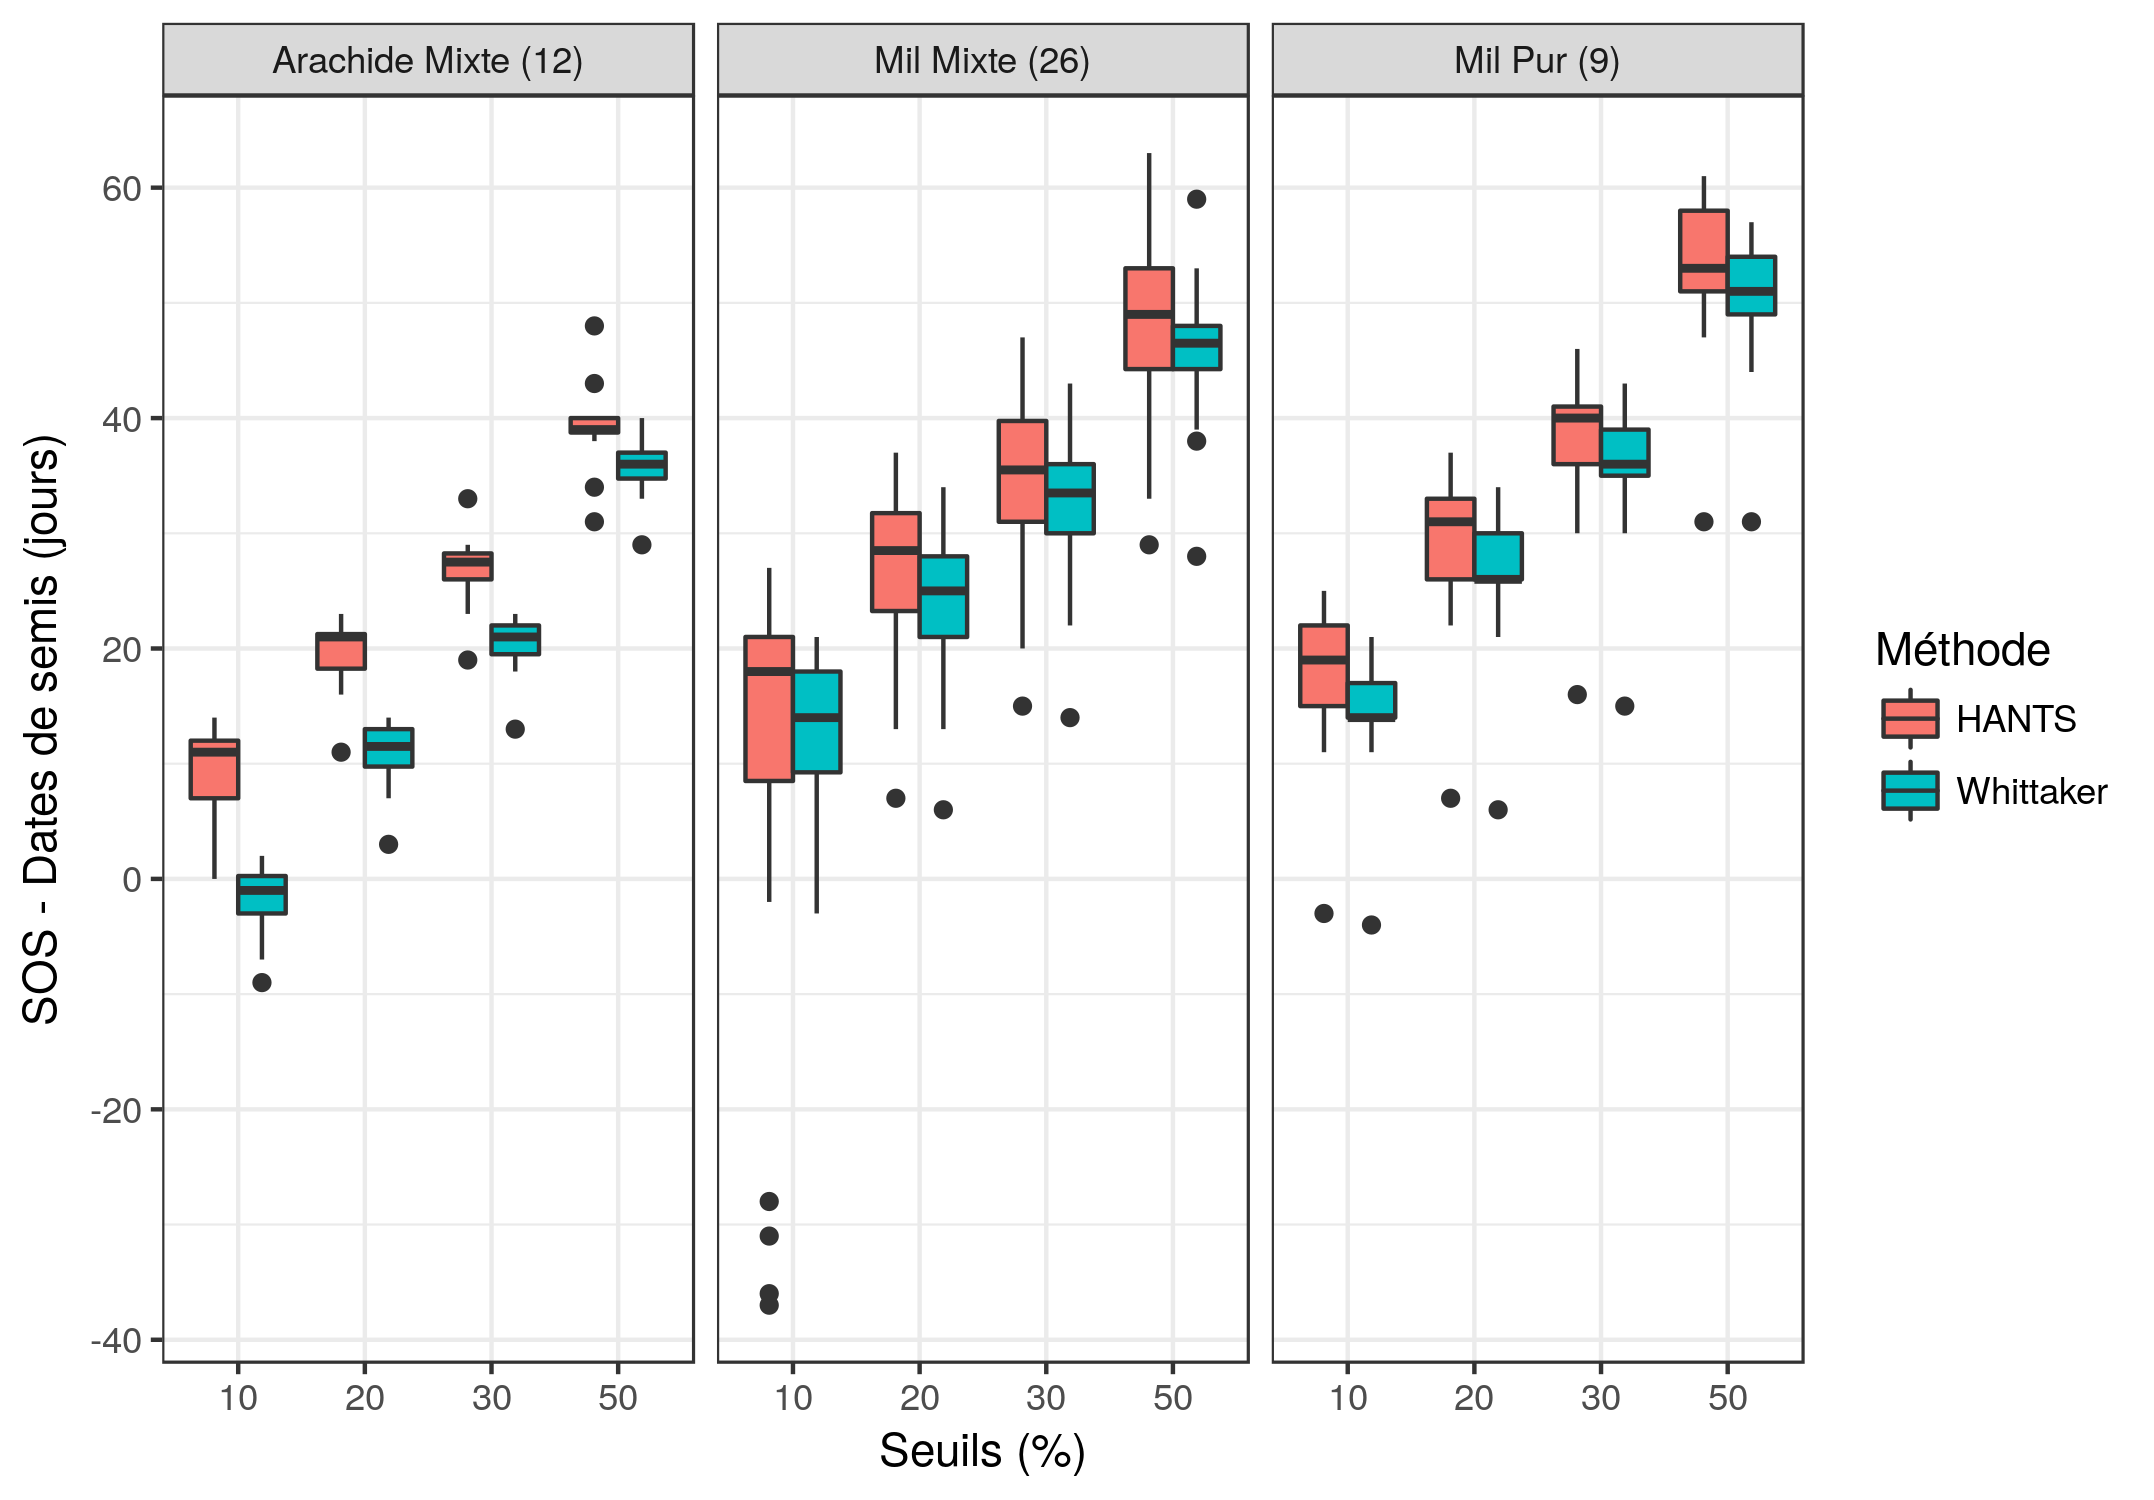
\includegraphics[scale=0.7]{resultats_discussions/SOS_Boxplot.png} 
 \end{center}
 \caption[Distribution des écarts entre SOS et dates de semis]{Boîtes à moustaches illustrant la distribution des écarts entre SOS estimés et dates de semis en fonction des systèmes de culture et des méthodes de lissage (\emph{Le nombre de parcelles est indiqué à la suite du système de culture})}
 \label{fig-sosboxplot}
\end{figure}

\begin{figure}[htbp]
 \begin{center}
  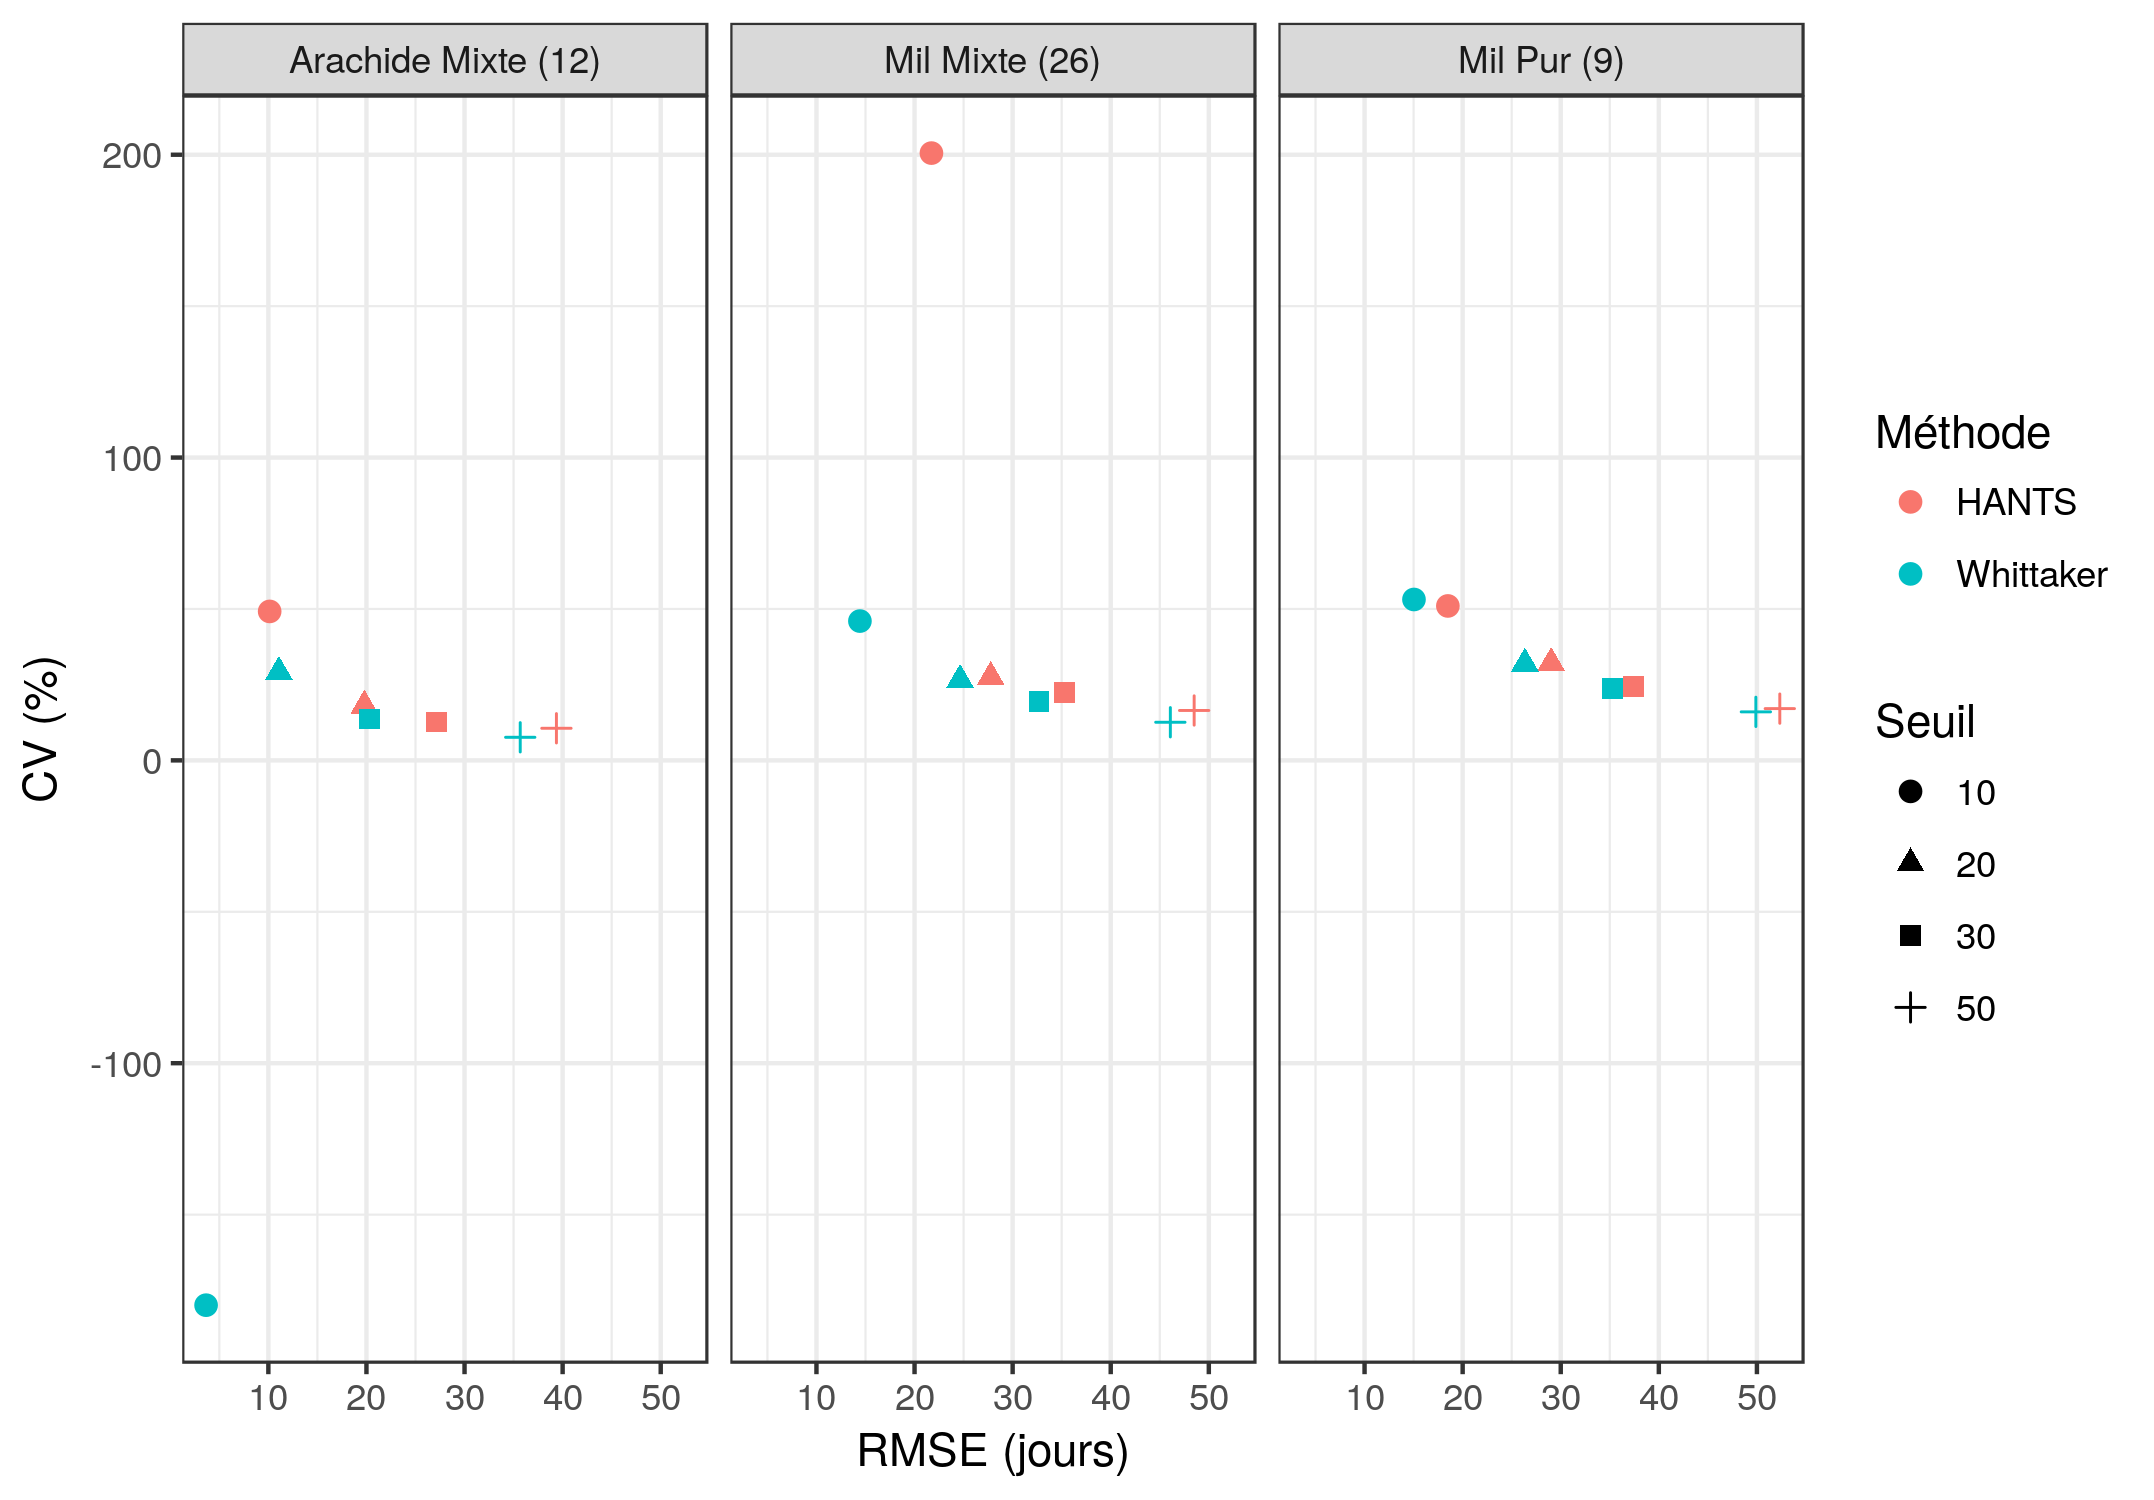
\includegraphics[scale=0.7]{resultats_discussions/SOS_RMSE_vs_CV.png} 
 \end{center}
 \caption[SOS -- RMSE vs CV]{Représentation du RMSE entre dates de semis et SOS estimés en fonction du coefficient de variation de leurs écarts par système de culture et méthode de lissage}
 \label{fig-sos-rmse-cv}
\end{figure}

\begin{figure}[htbp]
 \begin{center}
  \includegraphics[scale=0.7]{resultats_discussions/Spatial_SOS.png} 
 \end{center}
 \caption[Spatialisation des SOS]{Spatialisation des SOS extraits à l'échelle pixellaire (3 mètres) sur la zone d'application du lissage}
 \label{fig-spatial-sos}
\end{figure}

\paragraph{EOS}

\subsection{Estimation des rendements}
  
\section{Discussions}

\subsection{Sur l'extraction du SOS et du EOS}

\subsection{Sur l'estimation des rendements}
